\chapter{Spectrum Analyzer}
The specific target of this exploit, is the tool called the spectrum analyzer, which can be exploited through a buffer overflow.
The intended purpose of the spectrum analyzer is to identify potential problems with the connection through the cable, such as interference.
The spectrum analyzer is exposed to the local network, although on varying ports depending on particular cable modem.
It can usually be discovered by running NMAP on \mono{192.168.100.*}, see \cref{lst:nmap_command}, which redirects to the modem itself, often either on \mono{192.168.0.1} or \mono{192.168.1.1}.
In some cases the endpoint require credentials, but so far a default set has been seen working on every example, as shown in \appendixref{app:ExploredRouters}.

\begin{lstlisting}[language=sh,firstnumber=1,label={lst:nmap_command},caption={The NMAP request to find the Spectrum Analyser},float]
    nmap 192.168.100.0/24
\end{lstlisting}

\section{Overflowing the Registers}
Requests to the spectrum analyzer is sent as JSON through a websocket. An example of an intended request can be seen in \cref{lst:json_intended}.
\lstinputlisting[language=json,firstnumber=1,label={lst:json_intended},caption={An expected request.},float]{legit_request.json}

However, the JSON deserializer used in the spectrum analyzer, allocates a predefined amount of memory for each parameter, but will keep reading input parameters until a comma (,) is reached.
This can be exploited with a malicious request, like the one seen in \cref{lst:json_malicious}.
Here the fStartHz has a parameter value bigger than the allocated memory, and will therefore overflow and overwrite the registers.
To validate this, a json package with 200 A's as the fStartHz parameter can be sent through the serial port to the CM.
This will crash the modem and all register values will be displayed, showing that the program counter has changed to 0x41414141.
A more thorough walk-through of how to check this, is given in \appendixref{app:howto}.

\lstinputlisting[language=json,firstnumber=1,label={lst:json_malicious},caption={A malicious request.},float]{overflow_request.json}


\chapter{Exploiting \exploitname}
This section will describe how \exploitname can be exploited using return oriented programming.

\section{Architecture and Calling convention}
The eCos OS running on the CM are compiled with the O32 ABI convention which has some implications on how the vulnerability can be exploited. In this section we will describe the architecture, calling convention and OS to give a understanding of what exploit techniques we can use. These are the different registers and their purposes:

\begin{itemize}
    \item \textbf{\$a0 - \$a3} are registers used for parsing parameters.
    \item \textbf{\$t7 - \$t9} are caller saved register and also used as parameters if more than 4 is needed. Further are pushed to the stack.
    \item \textbf{\$v0 and \$v1} are used for return values.
    \item \textbf{\$s0 - \$s7} are callee saved registers.
    \item \textbf{\$fp} are the frame pointer but used as a s register under this calling convention.
    \item \textbf{\$sp} are the stack pointer.
    \item \textbf{\$ra} is the return address.   
\end{itemize}

As we see we have nine callee saved registers in total and the spectrum analyzer uses all 9 of them, which means that besides pushing the return address to the stack these nine registers is pushed and restored as well. This means that we have full control of program execution and these registers.
besides dictating how parameters are passed the convention also specifics how the stack should be extended and restored. As the frame pointer is used as a normal register it's not used for referencing variables in scope of the function instead the stack pointer is used. The stack pointer is further more only manipulate in the beginning and end of a function. In the beginning it will be counted down by the amount of bytes needed for the function and in the end the same value is added again. This means that the stack pointer is only being manipulate in a relative manner and never saved on the stack if we excluding kernel operations such as context switch.

\section{Limitations}
With the calling convention in mind we will now list how this implicates the exploitation techniques we can use. As the stack pointer is never pushed we cannot manipulate or read it meaning that we cannot leak the stack pointer or use stack pivoting at all. This makes stack execution impractical even thorough it is allowed by the OS. The firmware is statically linked and there is no such thing as global offset table and procedure linkage table meaning that wan be overwriten. This leaves us with one choise which is to use return oriented programing. Fortunately the firmware is not running with position independent execution and there is no address space layout randomization meaning that all addresses can be known before hand, and thous making return oriented programming convenient. Further more the firmware is statically linked with most of glibc available leaving us with a lot of gadgets.

\section{Return Oriented Programming}
As we have program counter control we can employ rop to run any existing code in the system, with our desired input variables inform of the s registers. Further more every time at gadget is used the s registers used in that function is restore meaning that we have control of all s registers doing the entire rop chain.
Although we are not able to execute our own code yet, through return oriented programming we are able to execute existing code on the system in a turing-complete manner and manipulate the system extensively.
This can be used to open a telnet server for external root access to the CM, allowing remote access to the system.
Through this telnet we can access a range of methods, but most importantly we can read and write memory addresses, and execute code from any memory address, including ones we have just written to.
These last steps varies from modem to modem, but one complete example can be found in \appendixref{app:technical_replication}.

\section{Unreachable gadgets}
Not all gadgets can be reached, as gadgets are just addresses sent over the websocket connection and we are forced to use the websocket text frame protocol we are limited to sending valid utf-8 character enforced by the browser.
For instance, the address 0x8080a864 can not directly be inserted in a WebSocket text frame, as it is not a valid UTF-8 character. The bytes sequence 0xf28080a864 can however be inserted, as 0xf2 means start new UTF-8 symbol with 3 trailing bytes 0x80, 0x80, 0xa8 and one ascii char 0x64. The following bytes cannot be present in any address used because of the utf-8 specification can never represent such byte in any way: 0xc0, 0xc1,0xf5, 0xf6, 0xf7, 0xf8, 0xf9, 0xfa, 0xfb, 0xfc, 0xfd, 0xfe, 0xff. Further more 0x2c and 0x00 cannot be used as 0x2c is ',' and is our json deliminator and 0x00 because we use strncpy. Be aware that when inserting a byte sequence such as 0xf28080a864 it has to be shifted one character so the address align with the position for the gadget, and the extra 0xf2 byte may now pe positioned in another register such as a s register making this register unusable doing the next gadget. Further more this also limits the values we can put on the stack fx. we cannot write the local ip 192.168.0.10 as it contains 192 which is an invalid character. In the cases were we need to call a function which is unreachable we can use other gadgets to add to registers together adding up to the desired value and jumping to that register instead.

% \begin{figure}
%   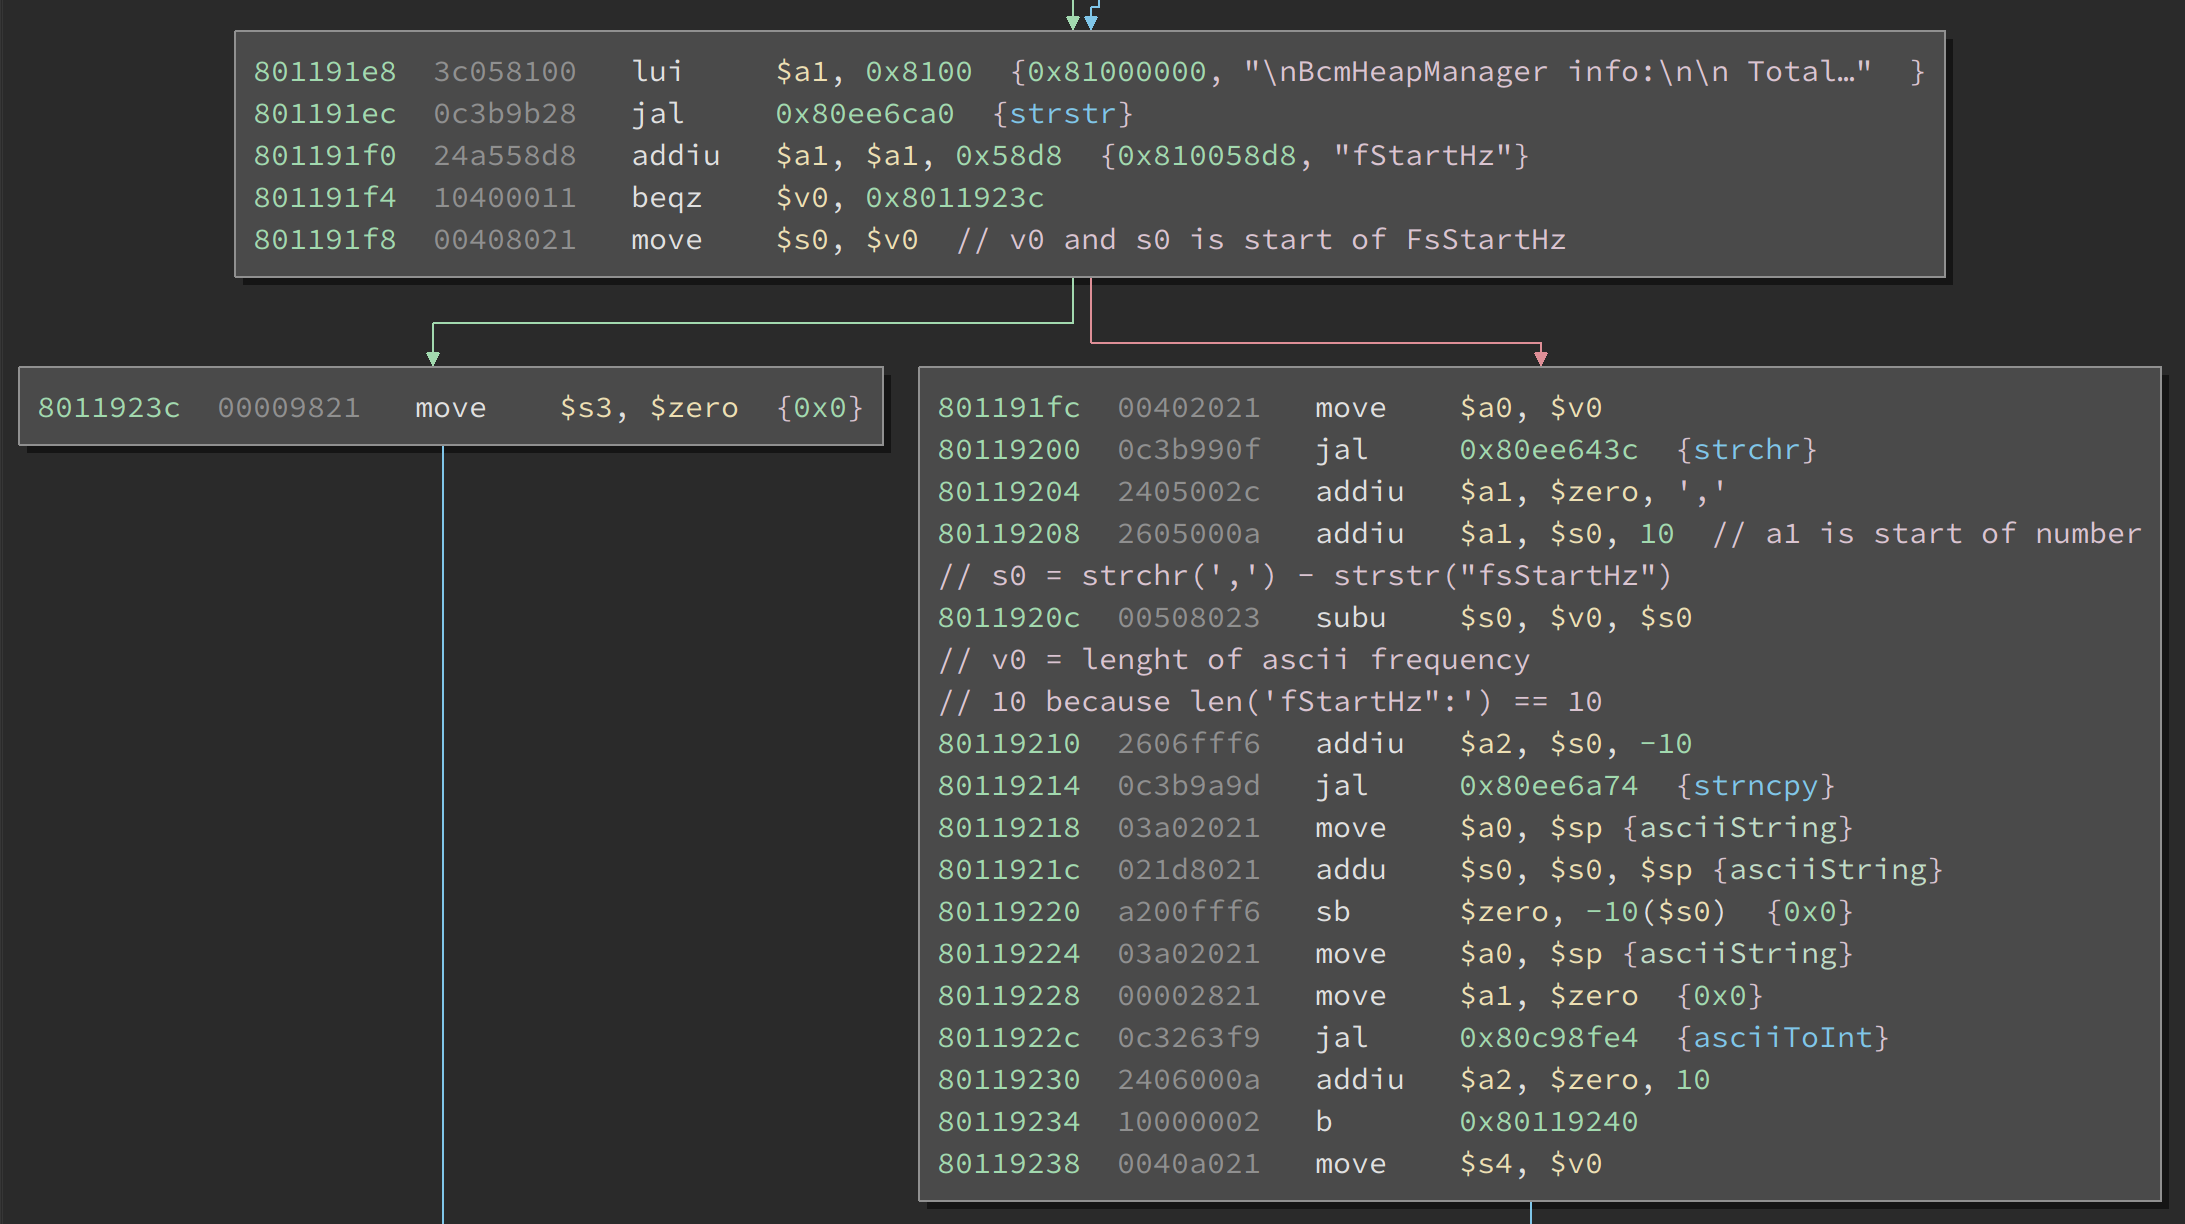
\includegraphics[width=\linewidth]{../graphics/spectrum.png}
%   \caption{Buffer overflow in beginning of stack as strncpy copies until it reaches a comma}
%   \label{fig:spectrum}
% \end{figure}
